\documentclass[12pt]{article}
\usepackage{tikz}
\usetikzlibrary{arrows.meta}

\begin{document}

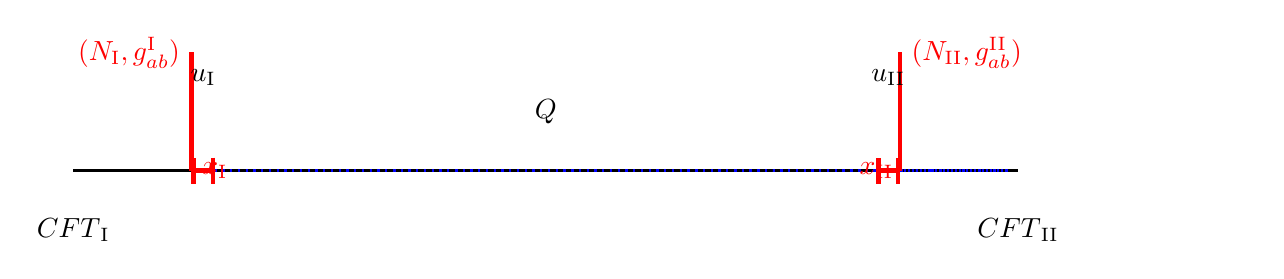
\begin{tikzpicture}[scale=1.5]
    % Draw the two CFTs
    \draw[thick] (-4,0) -- (4,0);
    \node at (-4,-0.5) {$\text{CFT}_\mathrm{I}$};
    \node at (4,-0.5) {$\text{CFT}_\mathrm{II}$};
    
    % Draw the interface brane Q
    \draw[blue,dotted,thick] (-3,0) .. controls +(4,0) and +(3,0) .. (3,0);
    \node at (0,0.5) {$Q$};
    
    % Mark the points of intersection
    \draw[red, ultra thick] (-3,0) -- (-3,1) node[left] {$(N_\mathrm{I},g^\mathrm{I}_{ab})$};
    \draw[red, ultra thick] (3,0) -- (3,1) node[right] {$(N_\mathrm{II},g^\mathrm{II}_{ab})$};
    
    % Mark the interface positions
    \node[red] at (-2.8,0) {$x_\mathrm{I}$};
    \node[red] at (2.8,0) {$x_\mathrm{II}$};
    
    % Mark the tension vector
    \draw [red, ultra thick,|-|] (-3,0) -- (-2.8,0);
    \node[above=1em] at (-2.9,0.4) {$u_\mathrm{I}$};
    
    \draw [red, ultra thick,|-|] (3,0) -- (2.8,0);
    \node[above=1em] at (2.9,0.4) {$u_\mathrm{II}$};
\end{tikzpicture}

\small Cartoon plot for the setup. The left and right bulk, denoted as \( N_\mathrm{I} \) and \( N_\mathrm{II} \) respectively, are dual to CFT_\mathrm{I} and CFT_\mathrm{II} respectively. The interface brane \( Q \) is in blue.

\end{document}